\documentclass[10pt]{beamer}
    
    \usetheme{glasgow}
    
    \usepackage{booktabs}
    \usepackage[scale=2]{ccicons}
    \usepackage{minted}
    \usepackage{bookmark}
    \usepackage[style=verbose]{biblatex}
    % \usepackage{filecontents}% to embed the file `myreferences.bib` in your `.tex` file
    % \begin{filecontents*}{refs.bib}
    %     @misc{schneider_understanding_nodate,
    %     title = {Understanding the {FDTD} {Method}},
    %     url = {https://eecs.wsu.edu/~schneidj/ufdtd/},
    %     author = {Schneider, John}
    % }
    % \end{filecontents*}

    \addbibresource{refs.bib}

    % \usepackage[noadjust]{cite}
    \usepgfplotslibrary{dateplot}
    
    \usemintedstyle{trac}
    
    % ($ (A)!r!(B) $) the location of images to be used
    \graphicspath{{src/}}
    
    %% Customisation
    % \newcommand{\V}[1]{\v} % vectors \v{c}
    % \renewcommand{\v}[1]{\mathbf{#1}} % vectors
    \newcommand{\ti}[1]{\tilde{#1}} % spectral representation
    \newcommand{\tnsr}[1]{\underline{\underline{#1}}}
    
    % Symbols
    \renewcommand{\O}{\omega}  % omega
    \newcommand{\E}{\varepsilon}  % epsilon
    \renewcommand{\u}{\mu}  % mu
    \newcommand{\p}{\rho}  % rho
    \newcommand{\x}{\times}  % times
    \renewcommand{\inf}{\infty}  % infinity
    \newcommand{\infint}{\int\limits_{-\inf}^\inf} % integral by R
    \newcommand{\e}{\mathrm{e}} % Straight-up exponential
    \renewcommand{\j}{{j}\mkern1mu} % Straight-up exponential
    \newcommand{\iu}{\mathrm{i}\mkern1mu}
    
    \newcommand\ddfrac[2]{\frac{\displaystyle #1}{\displaystyle #2}}
    
    \usepackage{animate}



%     % Define a the counter cnt. Used to identify files generated for use
% % with Gnuplot.
% \newcounter{cnt}
% \setcounter{cnt}{0}

% % Macro for drawing one frame of the F-distribution animation.
% \newcommand{\fdst}[4]{%
%     % shade the critical region tail
%     \draw[fill,orange]  (#1,0) -- plot[id=5\thecnt,domain=#1:5.5,samples=50]
%         function {#4*(x**(0.5*#2-1))*((1+#2*x/#3)**(-0.5*#2-0.5*#3))}
%             -- (5.5,0) -- cycle;

%     % draw the F distribution curve
%     \draw[color=blue!50!black,thick]
%         plot[id=f4\thecnt,smooth,domain=0:5.5,samples=100]
%         function {#4*(x**(0.5*#2-1))*((1+#2*x/#3)**(-0.5*#2-0.5*#3))};

%     % draw the F axis
%     \draw[->] (0,0) -- (6,0) node[right] {$F$};
%     % label the critical region boundary
%     \draw (#1,0) -- (#1,-0.02) node[below] {$#1$};
%     % label 0
%     \draw (0,0) -- (0,-0.02) node[below] {$0$};

%     % add some lables for degrees of freedom and alpha level
%     \draw (2,0.5) node[right] {$df_1 = #2$};
%     \draw (2,0.4) node[right] {$df_2 = #3$};
%     \draw (2,0.3) node[right] {$\alpha = 0.10$};

%     % draw the y axis
%     \draw[very thin,->] (0,0) -- (0,0.8);
% }


    \title{High Frequency Communication Systems}
    \subtitle{Lecture 7}
    \date{Spring 2021}
    \author{Hasan T Abbas \& Qammer H Abbasi}
    % \institute{}
    




\begin{document}

\maketitle

%%%%%%%%%%%%%%%%%%%%%%%%%%%%%%%%%%%%%%%%%%
%%%%%%%%%%%%%%%%%%%%%%%%%%%%%%%%%%%%%%%%%%
%%%%%%%%%%%%%%%%%%%%%%%%%%%%%%%%%%%%%%%%%%
\begin{frame}[fragile]
    \frametitle{Lecture Outline}
    \begin{outline}[itemize]
        \1 Antenna Arrays
        \1 Array Analysis
        \2 Uniform linear arrays 
        \2 Non-uniform arrays
    \end{outline}
\end{frame}
%%%%%%%%%%%%%%%%%%%%%%%%%%%%%%%%%%%%%%%%%%
%%%%%%%%%%%%%%%%%%%%%%%%%%%%%%%%%%%%%%%%%%
%%%%%%%%%%%%%%%%%%%%%%%%%%%%%%%%%%%%%%%%%%

\section{Antenna Arrays}




\begin{frame}
    \frametitle{Antenna Array Motivation}

    \begin{columns}[T]
        \begin{column}{.4\textwidth}
            \begin{outline}
                \1 In individual antenna elements, we can't control the radiation patterns
                \1 If we \textit{combine} two antenna elements, it is possible to change the pattern significantly
                \2 We call the new combined structure as an \textcolor{red}{antenna array}.
                \1 We achieve higher directivity using antenna arrays
            \end{outline}
        \end{column}
        \begin{column}{.6\textwidth}
            \begin{figure}[h!]
                \centering
                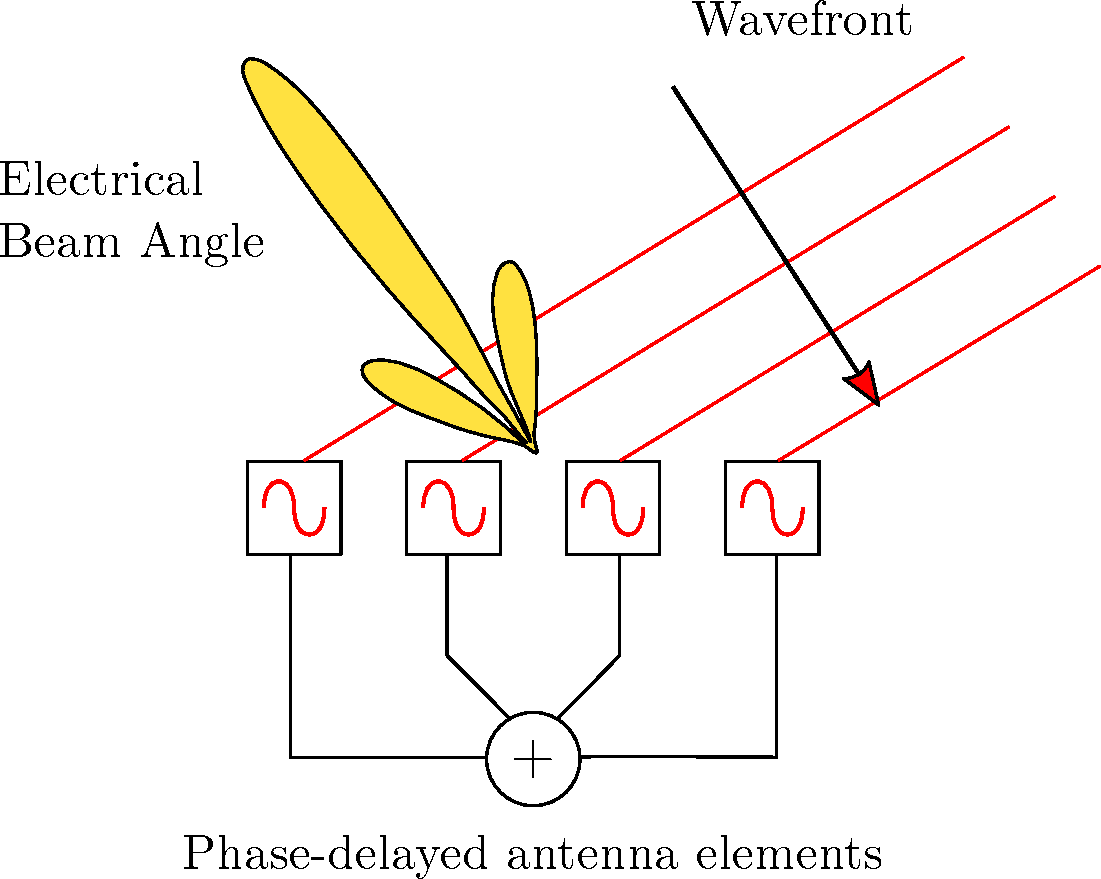
\includegraphics[width=0.95\textwidth]{antenna_array.pdf}
                \caption{Typical antenna array with phased elements.}
            \end{figure}
        \end{column}
    \end{columns}
        
\end{frame}



\begin{frame}
        \frametitle{Antenna Array Applications}
        \begin{columns}[T]
            \begin{column}{.4\textwidth}
                \begin{outline}
                    \1 Communications Applications
                    \2 The goal is to focus EM energy towards the target population (cars, people, cities etc.)
                    \3 Modern wireless communications using beamforming
                    \1 Radar - multiple target tracking
                    \2 We would like to focus the energy on the targets as they move
                \end{outline}
            \end{column}
            \begin{column}{.6\textwidth}
                \begin{figure}[h!]
                    \centering
                    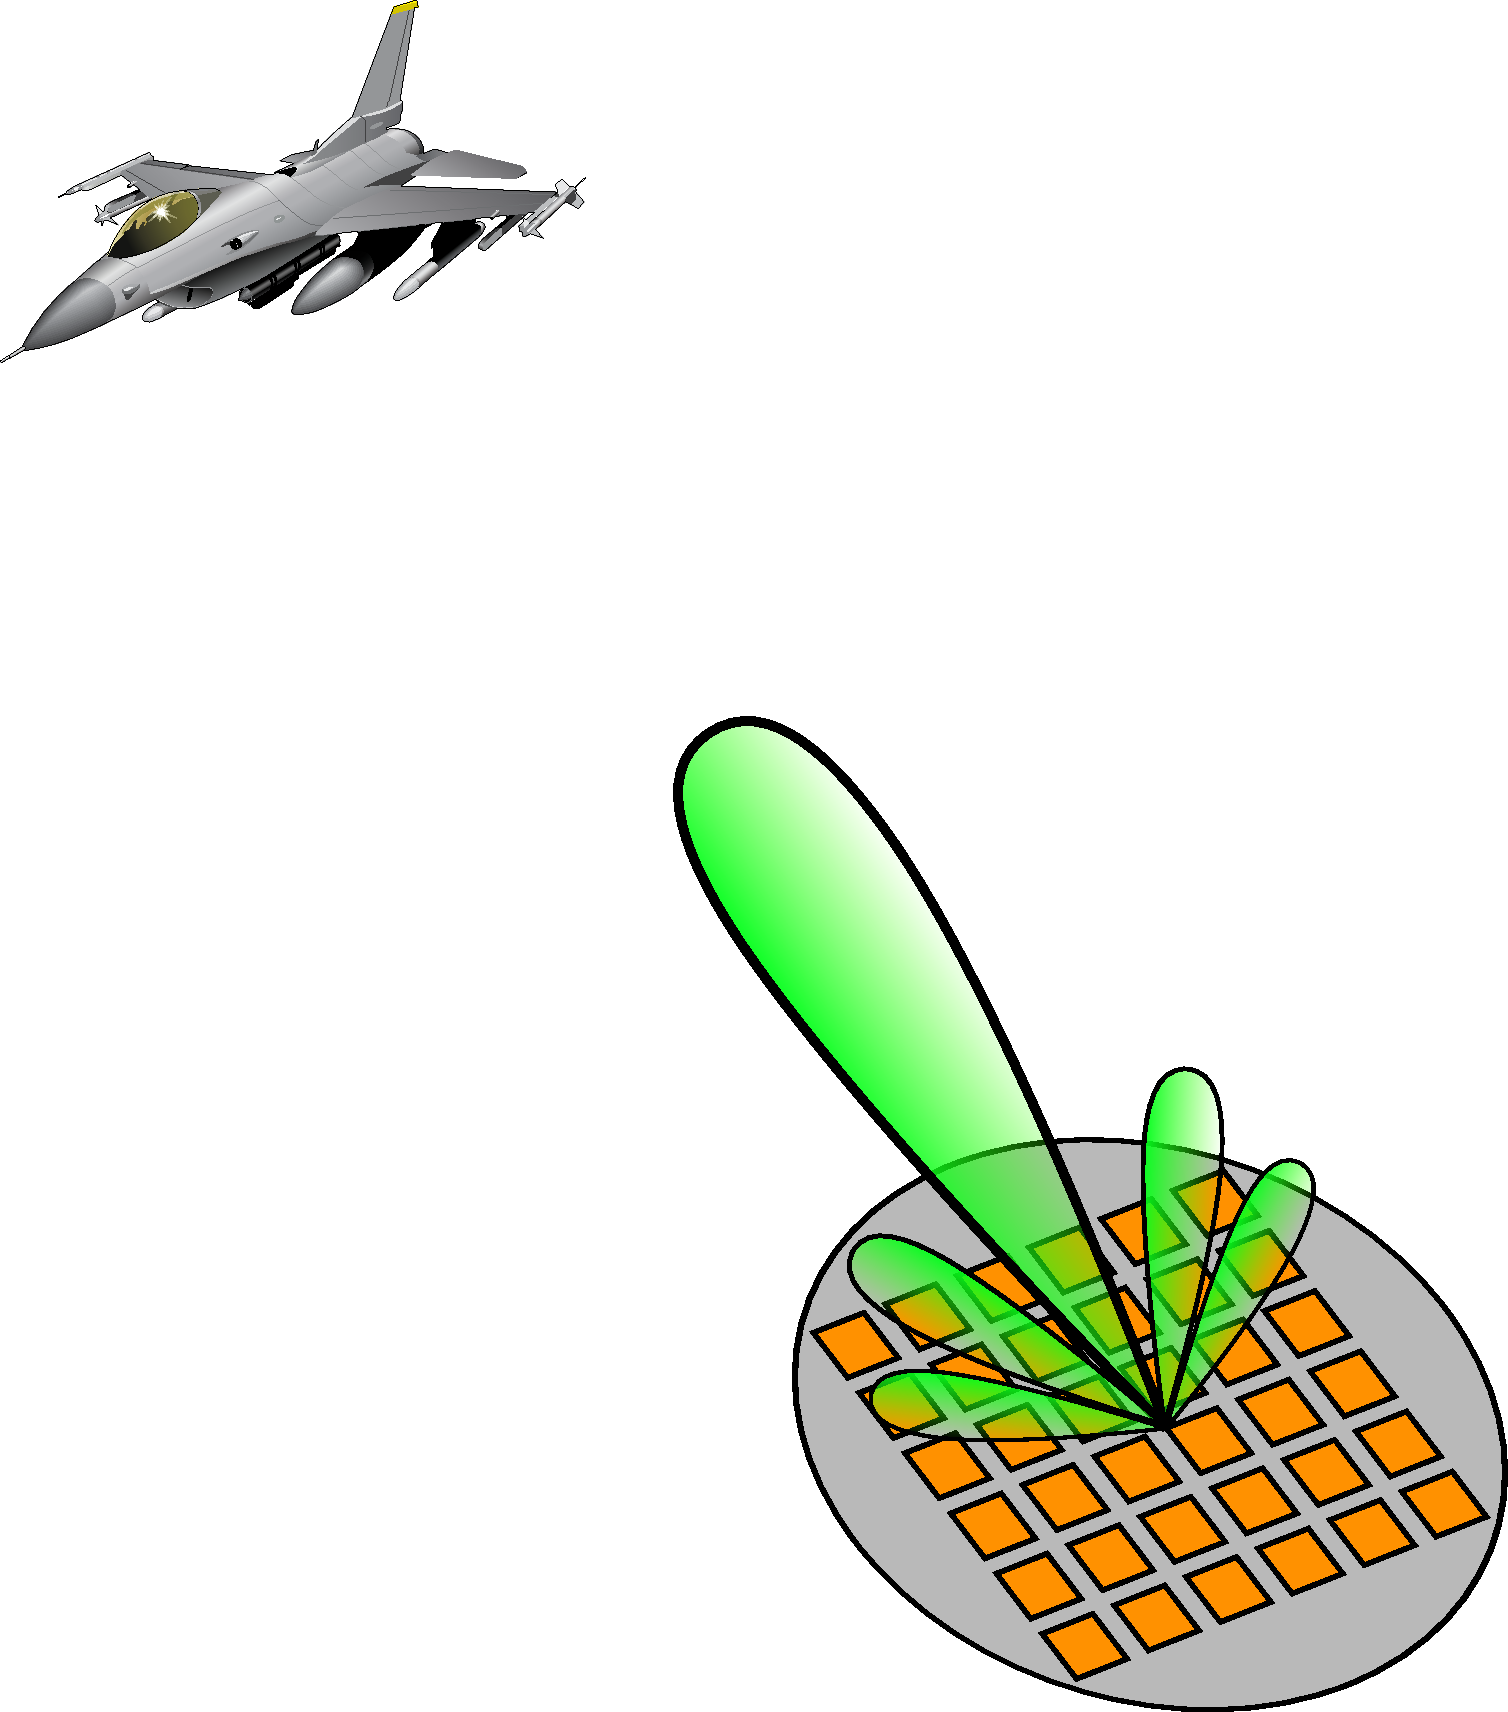
\includegraphics[width=0.65\textwidth]{arrays_motivation.pdf}
                    \caption{A Phased array antenna in RADAR based target tracking.}
                \end{figure}
            \end{column}
        \end{columns}

\end{frame}

\begin{frame}
    \frametitle{The Array element - point dipole}
    \begin{columns}[T] % align columns
        \begin{column}{.4\textwidth}
            \begin{outline}
                \1 Recall from the antenna introduction lecture, the field pattern of an infinitesimal dipole:
            \end{outline}
            \begin{align*}
                \va{E} {}=& \vu*{\gamma} \j k \eta I_0 l \frac{\exp(-\j k r)}{4 \pi r} \sin \gamma \nonumber \\
                &= \j k \eta \va{h} G(r)
            \end{align*}
            where $\va{h} = \vu*{\gamma} I_0 l \sin \gamma$ and $G(r)$ is the free-space Green function for a point source, $\exp(\j k r)/(4 \pi r)$
            \begin{outline}
                \1 We will use this as the antenna element
            \end{outline}
        \end{column}
        \begin{column}{.4\textwidth}
            \begin{figure}[B!]
                \centering
                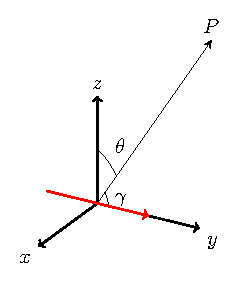
\includegraphics[width=.75\textwidth]{line_source.pdf}
            \end{figure}
            \begin{figure}[h!]
                \centering
                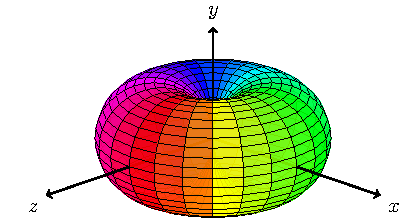
\includegraphics[width=.9\textwidth]{3d_pattern.pdf}
            \end{figure}
        \end{column}%
    \end{columns}
\end{frame}

\begin{frame}
    \frametitle{Obtaining a desired pattern}

    \begin{outline}
        \1 There are some factors that determine the desired radiation pattern
        \2 Array Geometry
        \2 Element Spacing
        \2 Element Excitation Amplitude
        \2 Pattern of individual element
    \end{outline}
The total field is given by:
\begin{align*}
    E_{total} {}=& \mathrm{Element \, \, Factor}  \times \mathrm{Array \, \, Factor}
\end{align*}
\end{frame}

\begin{frame}
    \frametitle{Two Element Array}
    \begin{columns}[T] % align columns
        \begin{column}{.6\textwidth}
            \begin{outline}
                \1 The simplest antenna array contains two elements
                \1 Two analyse an array, we start by using point sources as individual elements
                \2 The final pattern is obtained by multiplication
                \1 First, we will ignore the mutual coupling between elements.
                \1 Consider an array of two point sources separated by a distance $d$ on the $z$-axis.
            \end{outline}
            \begin{outline}
                \1 Assuming that both the antenna elements are excited by the current $I_1 = I_0 \exp (\j \alpha/2)$ and $I_2 = I_0 \exp (-\j \alpha/2)$ where $0 \le \alpha \le 2 \pi$.
            \end{outline}   
        \end{column}
        \begin{column}{.4\textwidth}
            \begin{figure}[T!]
                \centering
                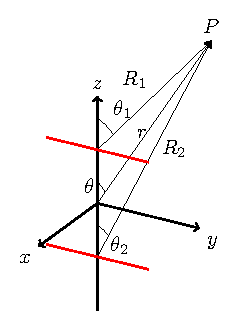
\includegraphics[width=.8\textwidth]{two_elements.pdf}
                \caption{Two point sources forming a basic antenna array.}
            \end{figure}

        \end{column}%
    \end{columns}
\end{frame}


\begin{frame}
    \frametitle{Two element array - Total Fields}
Neglecting any mutual coupling, we obtain the total fields by simple vector summation:
\begin{align*}
    \va{E_t} {}=& \va{E_1} + \va{E_2} \\
    &= \vu*{\gamma} \j k \eta \frac{I_{0} \ell}{4 \pi}\left\{\frac{\e^{-\j k R_{1}}}{R_{1}} \e^{+\j \alpha / 2} \sin \gamma_{1}+\frac{\e^{-\j k R_{2}}}{R_{2}} \e^{-\j \alpha / 2} \sin \gamma_{2}\right\}
 \end{align*}
    We use the \textit{far-field} approximation:
    \begin{align*}
        \gamma_1 \approx \gamma_2 \approx \gamma \\
        R_1 \approx r - \frac{d}{2} \cos \theta \\
        R_2 \approx r + \frac{d}{2} \cos \theta \\
       R_1 \approx R_2 \approx r (\mathrm{amplitude \, term})
    \end{align*}
\end{frame}

\begin{frame}
    \frametitle{Two element array - Total Fields}

    The total \textit{far-field} thus becomes:
    \begin{align*}
        \va{E_t} {}=& \vu*{\gamma} \j k \eta \frac{I_{0} \ell}{4 \pi r} \sin \gamma \left\{\e^{-\j k \frac{d}{2}\cos \theta } \e^{- \j \alpha / 2} + \e^{-\j k \frac{d}{2}\cos \theta } \e^{+\j \alpha / 2}\right\} \\
        &= \j k \eta \va{h} G(r) \left\{ \e^{\frac{k d cos \theta + \alpha}{2}} + \e^{-\frac{k d cos \theta + \alpha}{2}}\right\} \\
        &= \underbrace{\j k \eta \va{h} G(r)}_{Element \, Factor} \underbrace{2 \cos \left[\frac{1}{2}\left(k d \cos \theta + \alpha\right)\right]}_{Array \, Factor}
    \end{align*}
We can control and change the pattern by varying $d$ and $\alpha$, which are the spacing and phase shifts.
\end{frame}


\begin{frame}
    \frametitle{Example - Varying the pattern}

    Lets look at different cases where we consider different values of $d$ and $\alpha$.
    \begin{outline}
        \1 $\alpha = \ang{0}$ and $d = \lambda/4$, for which the array factor (AF) is
    \end{outline}
    \small
    \begin{align*}
        AF {}=& 2 \cos \left[ \frac{1}{2} \left( k d \cos \theta + \alpha  \right) \right] = 2 \cos \left(\frac{\pi}{4}\cos \theta \right)
    \end{align*}
    \normalsize
\begin{figure}[T!]
    \centering
    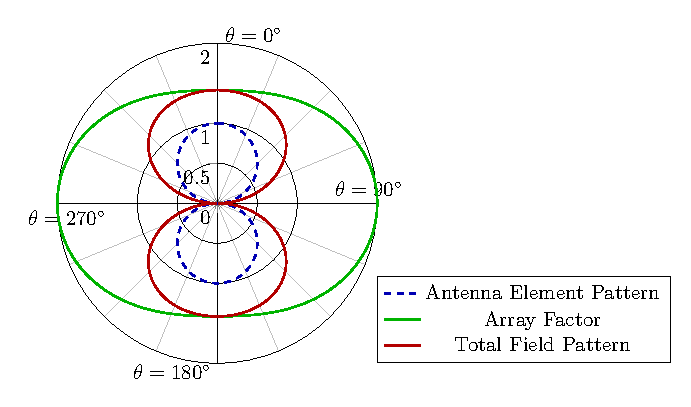
\includegraphics[width=.55\textwidth]{total_pattern_d_quarter_alpha_0.pdf}
    \caption{The total field pattern for $\alpha = \ang{0}$ and $d = \lambda/4$.}
    \label{fig:antenna_array}
\end{figure} 
\end{frame}   

\begin{frame}
    \frametitle{Example - Varying the pattern}

    \begin{outline}
        \1 Now looking at $\alpha = \ang{90}$ and $d = \lambda/4$, for which the array factor (AF) is
    \end{outline}
    \small
    \begin{align*}
        AF {}=& 2 \cos \left[ \frac{1}{2} \left( k d \cos \theta + \alpha  \right) \right] = 2 \cos \left(\frac{\pi}{4}\cos \theta + \frac{\pi}{4}\right)
    \end{align*}
    \normalsize
\begin{figure}[T!]
    \centering
    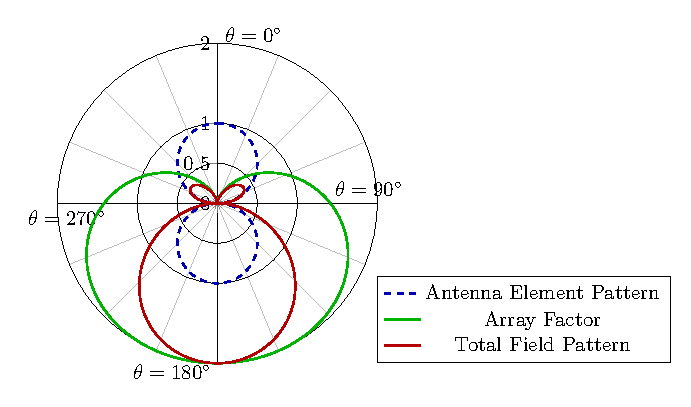
\includegraphics[width=.55\textwidth]{total_pattern_d_quarter_alpha_90.pdf}
    \caption{The total field pattern for $\alpha = \ang{90}$ and $d = \lambda/4$.}
    \label{fig:antenna_array}
\end{figure}  

\end{frame}

\begin{frame}
    \frametitle{Example - Varying the pattern}

    \begin{outline}
        \1 Now looking at $\alpha = \ang{-90}$ and $d = \lambda/4$, for which the array factor (AF) is
    \end{outline}
    \small
    \begin{align*}
        AF {}=& 2 \cos \left[ \frac{1}{2} \left( k d \cos \theta + \alpha  \right) \right] = 2 \cos \left(\frac{\pi}{4}\cos \theta - \frac{\pi}{4}\right)
    \end{align*}
    \normalsize
\begin{figure}[T!]
    \centering
    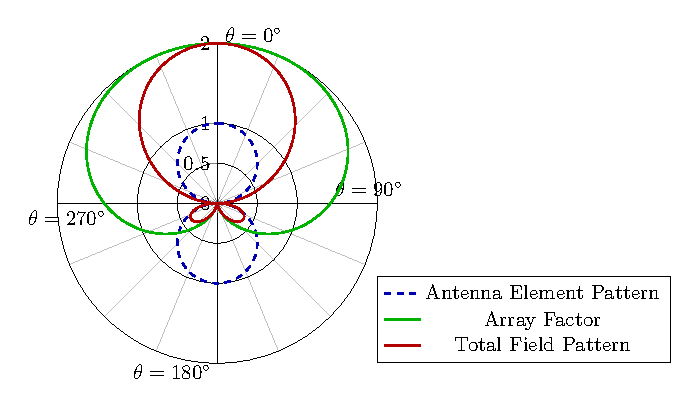
\includegraphics[width=.55\textwidth]{total_pattern_d_quarter_alpha_minus90.pdf}
    \caption{The total field pattern for $\alpha = \ang{-90}$ and $d = \lambda/4$.}
    \label{fig:antenna_array}
\end{figure}  

\end{frame}


\section{N-Element Arrays}

\begin{frame}
    \frametitle{N-Element Uniform Array}
    \begin{columns}[T] % align columns
        \begin{column}{.6\textwidth}
            \begin{outline}
                \1 A uniform array consists of equally spaced and identical elements
                \2 All elements are excited with \textit{same} amplitude
                \2 However, the elements have a \textcolor{red}{progressive} phase shift.
                \1 As before, the total field is the vector sum of the individual elements:
            \end{outline}
\begin{align*}
    \va{E}_T {}=& \va{E}_0 + \va{E}_1 + \va{E}_{-1} + \va{E}_2 + \va{E}_{-2} + \dots \\
    &= \j k \eta \va{h} G(r) \left( 1 + \e^{\j \psi} + \e^{-\j \psi} + \e^{2\j \psi}+ \e^{-2\j \psi} + \dots \right) 
 \end{align*}  
 where $\psi = k d \cos \theta + \alpha$
        \end{column}
        \begin{column}{.5\textwidth}
            \begin{figure}[T!]
                \centering
                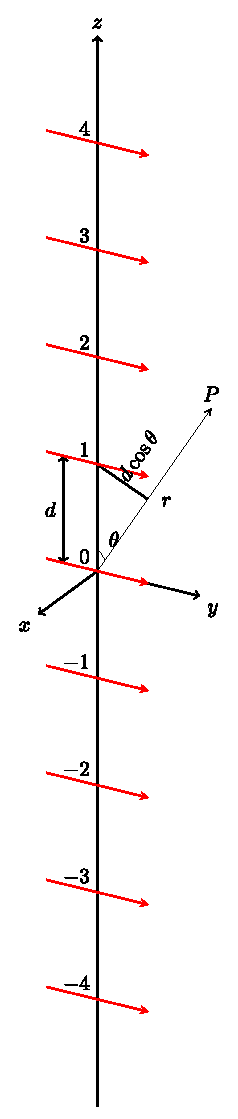
\includegraphics[height=1.3\textwidth]{N_elements.pdf}
            \end{figure}
        \end{column}%
    \end{columns}
\end{frame}

\begin{frame}[fragile]
    \frametitle{The Array Factor of N element array}
Continuing, we can write the AF as:
\small
\begin{equation}
    AF=\sum_{n=-N'}^{N'} \e^{\j n \psi} \quad \text { where } N' =\frac{(N-1)}{2}
    \label{eq:N_element_AF}
\end{equation}
\normalsize
We can also express \eqref{eq:N_element_AF} as:
\small
\begin{equation}
    AF \e^{\j n \psi} =\sum_{n=-N'}^{N'} \e^{\j (n+1) \psi}
    \label{eq:N_element_AF_1}
\end{equation}
\normalsize
From  \eqref{eq:N_element_AF_1} and \eqref{eq:N_element_AF} we get:
\small
\begin{align*}
    AF {}=& \frac{\e^{\j (N+1)\frac{\psi}{2}} - \e^{-\j (N-1)\frac{\psi}{2}}}{\e^{\j \psi} - 1} \\
    {}=& \frac{\e^{\j \psi/2 }}{\e^{\j \psi/2 }} \left[\frac{\e^{\j N\psi/2} - \e^{-\j N\psi/2}}{\e^{\j \psi/2} - \e^{-\j \psi/2}}\right]
\end{align*}
\normalsize
\begin{tcolorbox}[colback=blue!5]
    \begin{align*}
        AF {}=& \frac{\sin N \psi/2 }{\sin \psi/2 } \text { where } \psi =k d \cos \theta + \alpha
    \end{align*}
  \end{tcolorbox}
\end{frame}


\begin{frame}
    \frametitle{Visualising the N Element Array Factor}
Noting that the above expression resembles a \textcolor{red}{sinc} function, we can extend this to find the AF of any discrete array made of uniformly spaced elements. A major difference, however is the sidelobes don't decay with the increasing function argument.

In general, we plot the AF in the normalised form (divide by $N$).

\begin{figure}[h!]
    \centering
    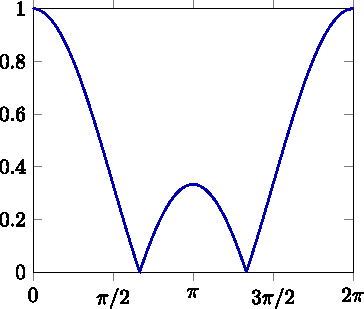
\includegraphics[width=.4\textwidth]{sinc.pdf}
    \caption{The normalised AF of a 3 element array.}
    \label{fig:3_element}
\end{figure} 
\end{frame}


\begin{frame}
    \frametitle{Some observations}

    \begin{columns}[T] % align columns
        \begin{column}{.6\textwidth}
            \begin{outline}
                \small
                \1 As $N $ increases, the main lobe narrows
                \1 We get more side lobes in one period of $AF$ as $N$ increases
                \1 The width of the minor/side lobes is $2\pi/N$
                \1 The side lobe height decreases as we increase $N$
                \1 $AF $ is symmetric about $\pi$ 
                \1 We also see that the peak value occurs at $\psi =\pm 2 n \pi$ for $n = 0,1,2, \dots$
                \1 The nulls occur at $\psi =\pm 2 n \pi/N$
                \1 The side lobe level is defined as:
            \end{outline}
\begin{align*}
    \text{SLL} {}=& \frac{\text{Max side lobe value}}{\text{Max Main lobe value}}
\end{align*}
        \end{column}
        \begin{column}{.5\textwidth}
            \begin{figure}[T!]
                \centering
                \subfloat[$N=5$]{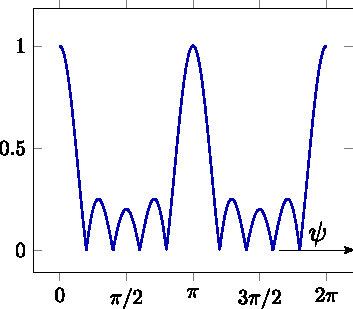
\includegraphics[width=1.05in]{sinc_5.pdf}
                \label{fig:field_at_20}}
                \\
                \subfloat[$N=10$]{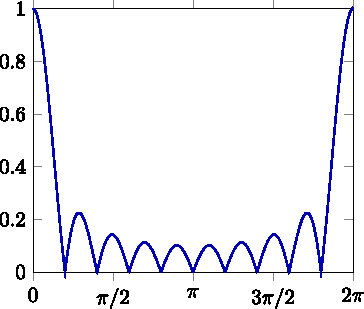
\includegraphics[width=1.05in]{sinc_10.pdf}
                \label{fig:field_at_60}}
                \caption{Array factors for $5$ and $10$ element uniform array.}
                \label{fig:E_z fields}
              \end{figure}
        \end{column}%
    \end{columns}
    \normalsize
\end{frame}

\begin{frame}
    \frametitle{Example - A 4 element array}
A four-element ($N =4$), uniformly excited, equally spaced array. The spacing $d$ is $\lambda/2$ and the interelement phasing $\alpha$ is $\ang{90}$.

\begin{figure}[h!]
    \centering
    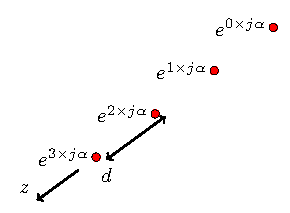
\includegraphics[width=.3\textwidth]{4_elements.pdf}
    \caption{A four element antenna array.}
    \label{<label>}
\end{figure}
    The normalised array factor is given by:
    \begin{align*}
        AF {}=& 1/4\frac{\sin 4 \psi/2 }{\sin \psi/2 } \text { where } \psi =\frac{2 \pi}{\lambda} \frac{\lambda }{2} \cos \theta + \ang{90}
    \end{align*}

\end{frame}

\begin{frame}
    \frametitle{4 Element Array - Pattern}
    \begin{columns}[T] % align columns
        \begin{column}{.7\textwidth}
            \begin{outline}
                \1 The linear plot is done as before
                \1 We can plot the corresponding polar plot by \textit{translating} peaks and main and side lobes
                \1 We first \textit{shift} the polar plot by an amount $\alpha$
                \2 One period of the $AF$ is considered
            \end{outline}
The direction of the main beam in the polar plot is found as:
\begin{align*}
    \psi {}=& k d \cos \theta + \alpha \\
    \theta {}=& \arccos \frac{\psi - \alpha }{k d} \\
    \theta_0 {}=& \arccos \left(\frac{0 - \pi/2 }{\pi}\right) = \ang{120}
\end{align*}
        \end{column}
        \begin{column}{.5\textwidth}
            \begin{figure}[t!]
                \centering
                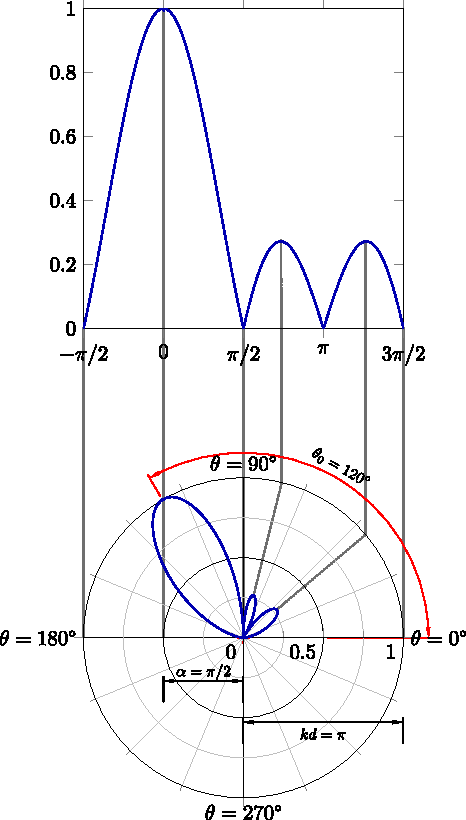
\includegraphics[height=1.2\textwidth]{Linear_polar_N_4_d_half_alpha_90.pdf}
            \end{figure}
        \end{column}%
    \end{columns}
\end{frame}

\begin{frame}
    \frametitle{Pattern Beamwidth}
    \begin{columns}[T] % align columns
        \begin{column}{.6\textwidth}
            In general there are two extreme cases which are sometimes used:
            \begin{outline}[enumerate]
                \1 Broadside $(\theta_0 = \ang{90})$ when $\alpha = 0$
                \1 Endfire $(\theta_0 = \ang{0} \text{or} \, \ang{180})$ when $\alpha = \pm k d$
            \end{outline}
The array pattern is often characterised by \textit{beamwidth between first nulls}. Knowing that the nulls occur at:
\small
\begin{align*}
    N \psi_{FN} /2 {}=& \pm \pi \\
    \text{For broadside array,} \quad \frac{N}{2} \frac{2\pi}{\lambda} d \cos \theta_{FN}  {}=& \pm \pi \\
    \theta_{FN} {}=& \arccos \left(\pm \frac{\lambda}{N d}\right)
\end{align*}
The BWFN is:
\begin{align*}
    BWFN {}=& \left| \theta_{\text{FN, left}} - \theta_{\text{FN, right}} \right|
\end{align*}
\normalsize
        \end{column}
        \begin{column}{.5\textwidth}
            \begin{figure}[t!]
                \centering
                \subfloat[Broadside]{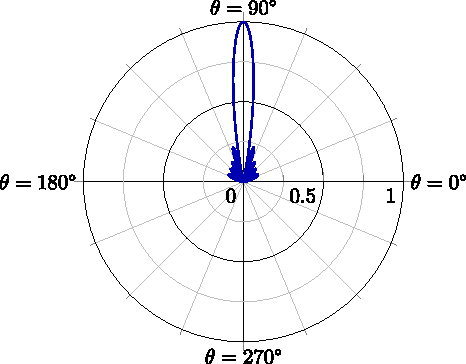
\includegraphics[width=1.25in]{broadside.pdf}
                \label{fig:field_at_20}}
                \\
                \subfloat[Endfire]{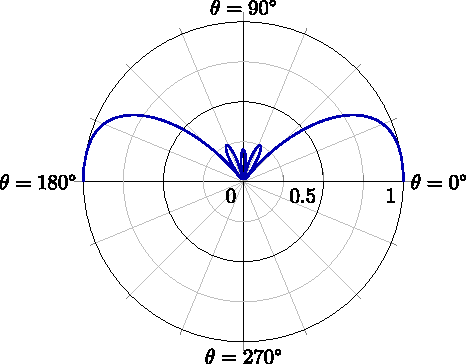
\includegraphics[width=1.25in]{endfire.pdf}
                \label{fig:field_at_80}}
              \end{figure}
        \end{column}%
    \end{columns}


\end{frame}


\begin{frame}
    \frametitle{Improving the Endfire Array}
For practical applications, we require a single pencil beam. To achieve it in the end-fire configuration, one of the ways to generate a single lobe is to use a backing ground plane. Another way to do this is to slightly decrease the element spacing below $\lambda/2$.

\begin{columns}[T] % align columns
    \begin{column}{.7\textwidth}
Some of the famous antennas such as the \textit{Yagi-Uda} implements this. The \textit{Hansen-Woodyard} endfire array also does it by introducing an \textcolor{red}{excess phase delay}:
\small
\begin{align*}
    \alpha {}=& \pm \left(k d + \delta \right)
\end{align*}
The end expressions for \textit{Hansen-Woodyard} array are:
\begin{align*}
    d {}<& \frac{\lambda}{2} \left(1 - \frac{1}{N}\right) \\
    \alpha {}=& \pm \left( k d + \frac{\pi }{N}\right)
\end{align*}
    \end{column}
    \begin{column}{.4\textwidth}
        \begin{figure}[t!]
            \centering
            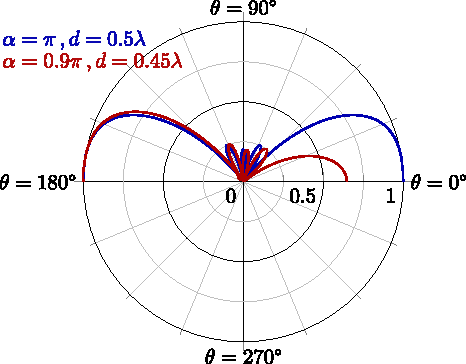
\includegraphics[width=.95\textwidth]{endfire_two.pdf}
            \caption{Slight change of the phase}
          \end{figure}
    \end{column}%
\end{columns}
\end{frame}

\begin{frame}
    \frametitle{Example - The Hanson-Woodyard Array}
Considering an example, where a five-element Hansen Woodyard has element spacing $d  = 0.37 \lambda$ and the element-element phase shift, $\alpha = 0.94 \pi$. Lets find the radiation pattern.

\begin{figure}[h!]
    \centering
    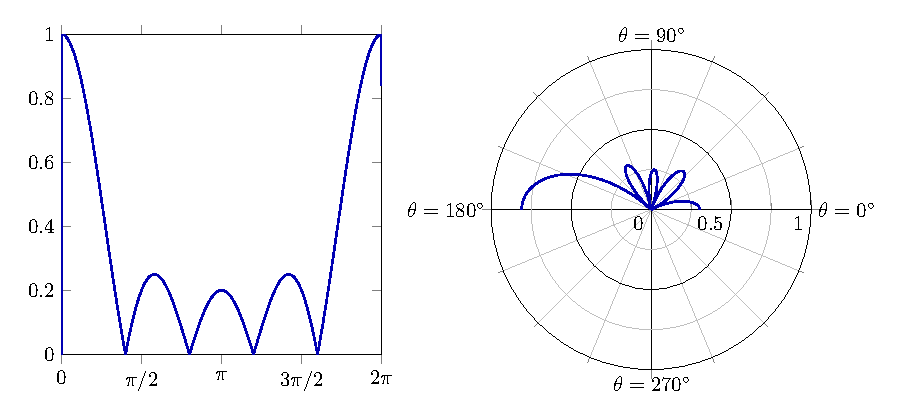
\includegraphics[width = .9 \textwidth]{Hansen Woodyard.pdf}
    \caption{The side by side plots of the linear and polar patterns of a Hansen Woodyard array.}
\end{figure}
\end{frame}


\begin{frame}
    \frametitle{Non-uniformly Excited Arrays}
The sidelobes can be further truncated using \textit{non-uniform} excitation on the elements. The $AF$ can now be written as a polynomial in terms of $Z = \e^{\j \psi}$:
\begin{align*}
    AF {}=& \sum_{n = 0}^{N-1} A_n \e^{\j n \psi} = \sum_{n = 0}^{N-1} A_n Z_n
\end{align*}

The current amplitudes $A_n$ are real-valued and different for each $n$.

Lets plot the array patterns for a five-element broadside array.

\end{frame}


\begin{frame}
    \frametitle{Triangular Array}
    \begin{figure}[!htbp]
        \centering
        \subfloat[]{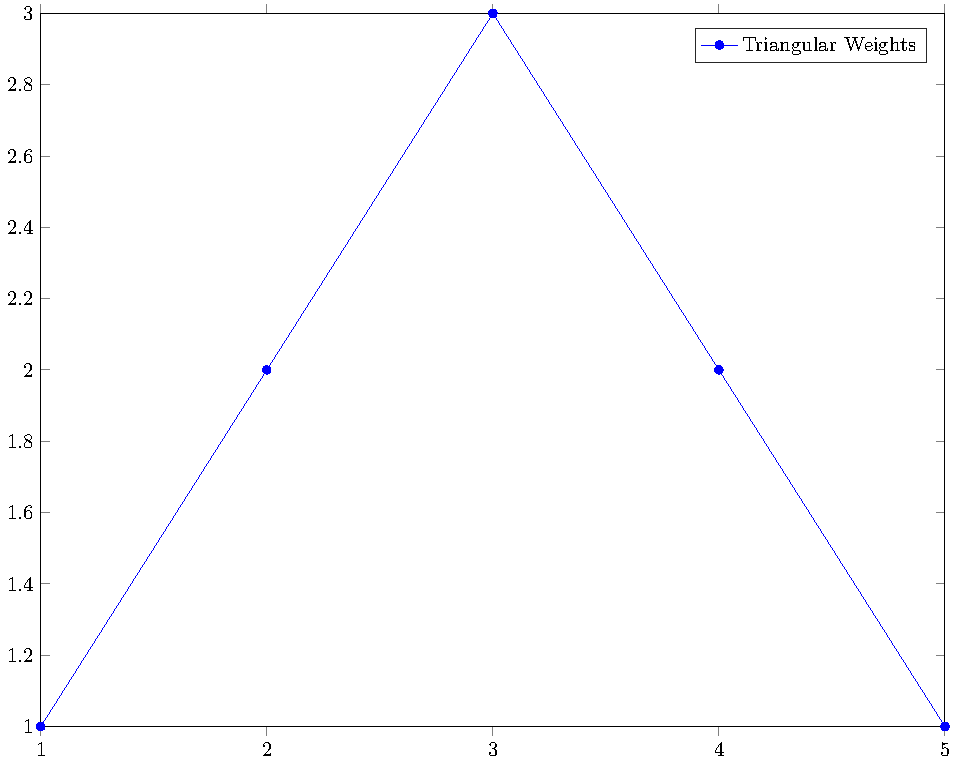
\includegraphics[width=.45\textwidth]{triangular_dist.pdf}
        \label{fig:field_at_20}}
        \hfil
        \subfloat[]{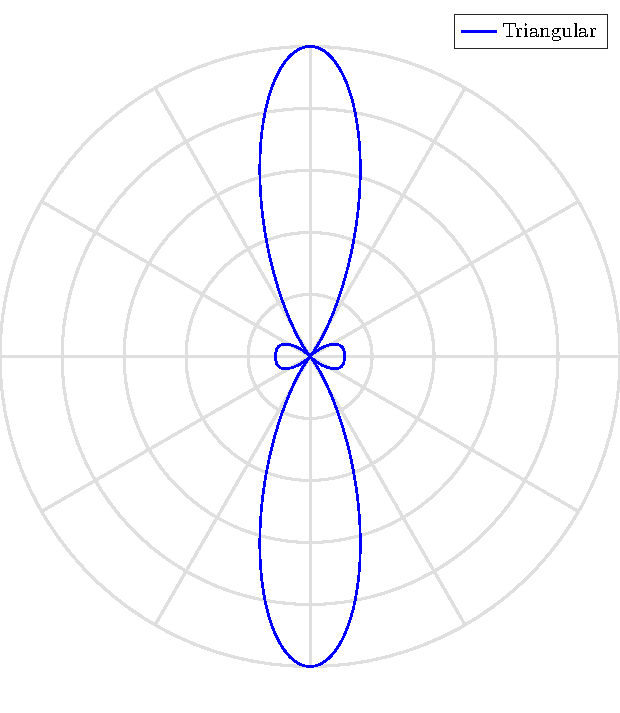
\includegraphics[width=.45\textwidth]{triangular.pdf}
        \label{fig:field_at_60}}
      \end{figure}
\end{frame}

\begin{frame}
    \frametitle{Binomial Array}
    \begin{figure}[!htbp]
        \centering
        \subfloat[]{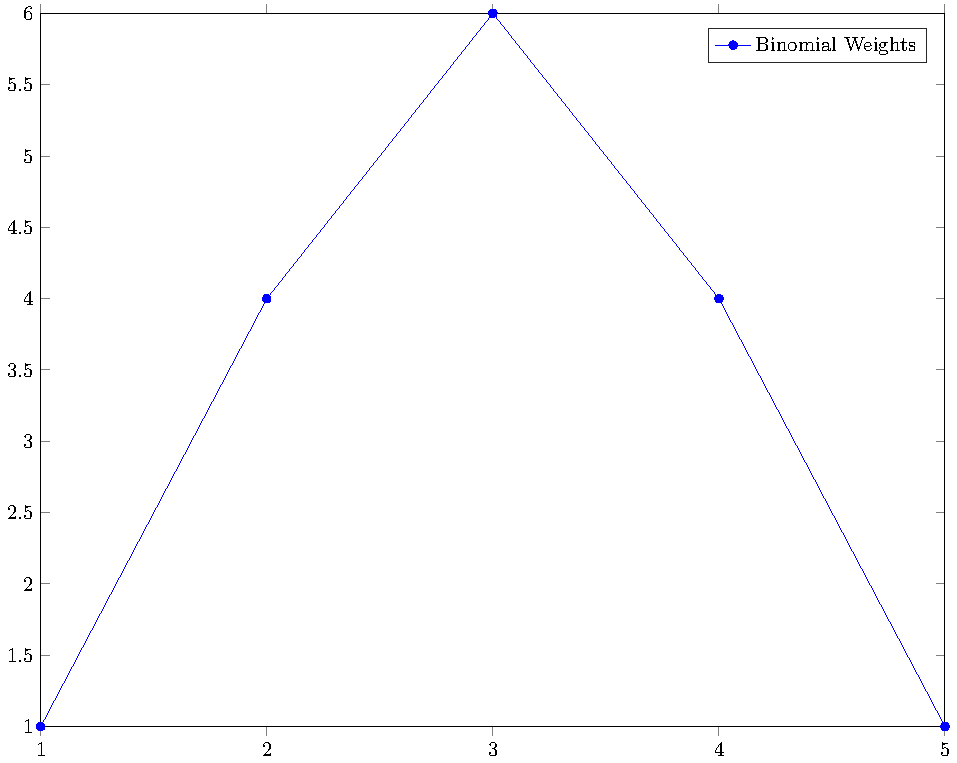
\includegraphics[width=.45\textwidth]{binomial_dist.pdf}
        \label{fig:field_at_20}}
        \hfil
        \subfloat[]{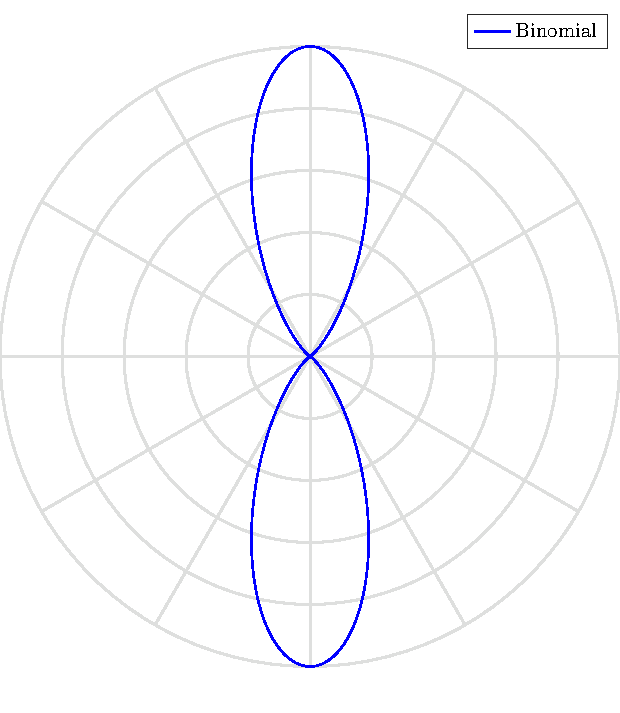
\includegraphics[width=.45\textwidth]{binomial.pdf}
        \label{fig:field_at_60}}
      \end{figure}
\end{frame}

\begin{frame}
    \frametitle{Dolph-Chebyshev Array}
    \begin{figure}[!htbp]
        \centering
        \subfloat[]{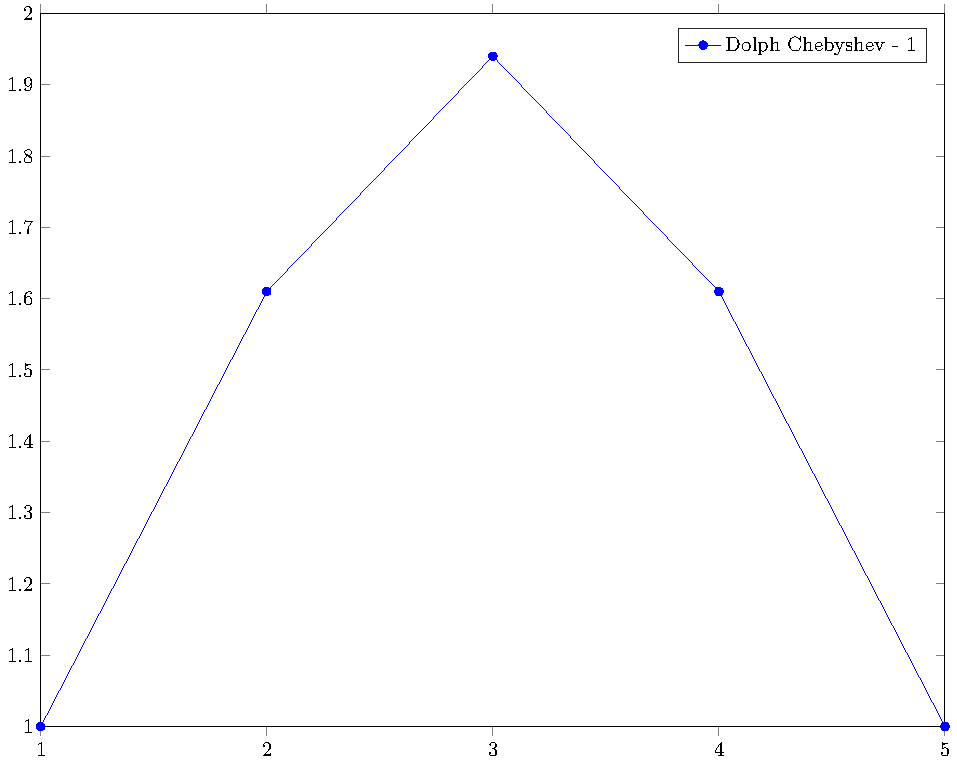
\includegraphics[width=.45\textwidth]{dc_dist.pdf}
        \label{fig:field_at_20}}
        \hfil
        \subfloat[]{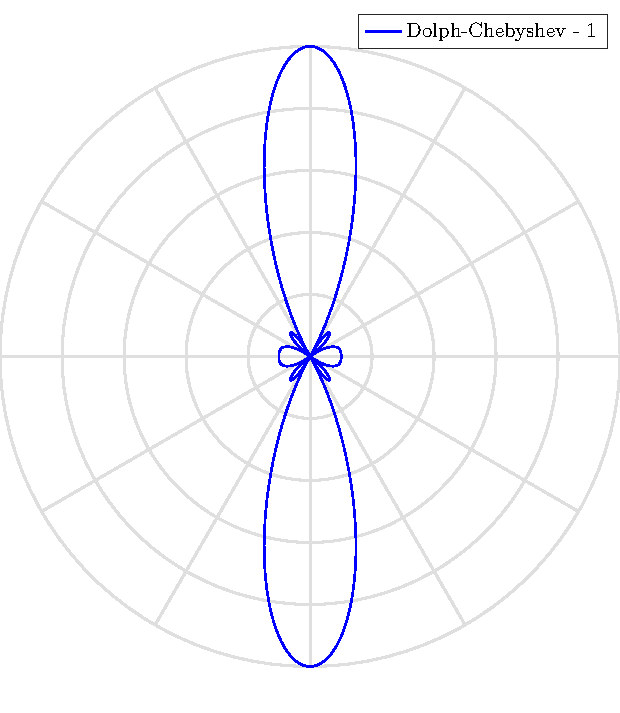
\includegraphics[width=.45\textwidth]{dc.pdf}
        \label{fig:field_at_60}}
      \end{figure}
\end{frame}

\begin{frame}
    \frametitle{Dolph-Chebyshev-2 Array}
    \begin{figure}[!htbp]
        \centering
        \subfloat[]{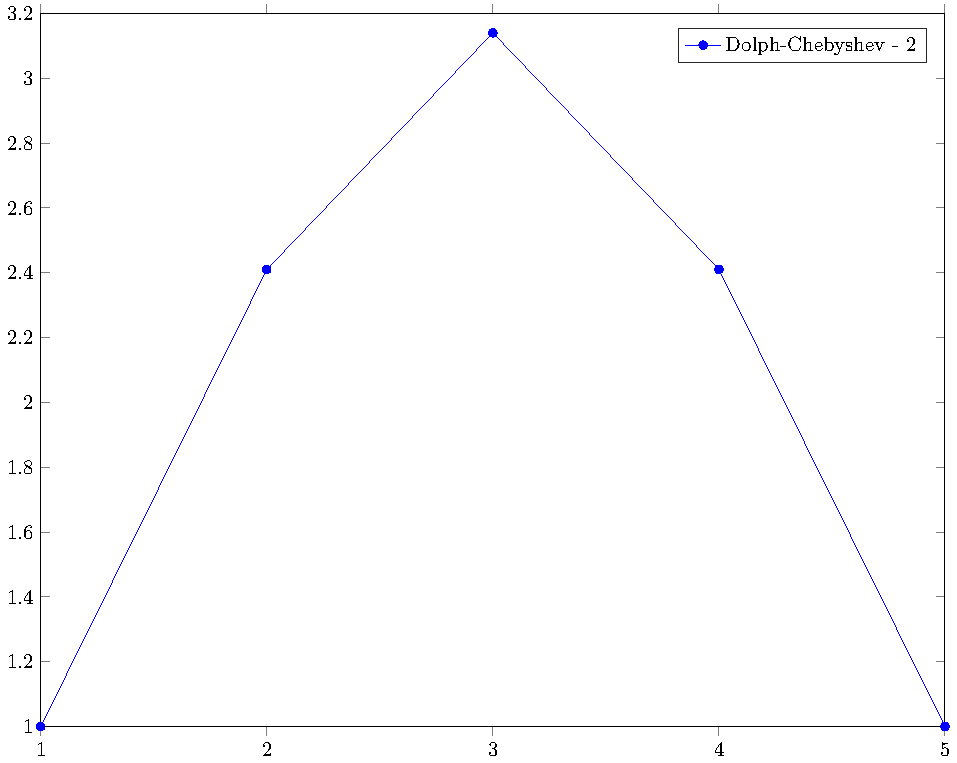
\includegraphics[width=.45\textwidth]{dc2_dist.pdf}
        \label{fig:field_at_20}}
        \hfil
        \subfloat[]{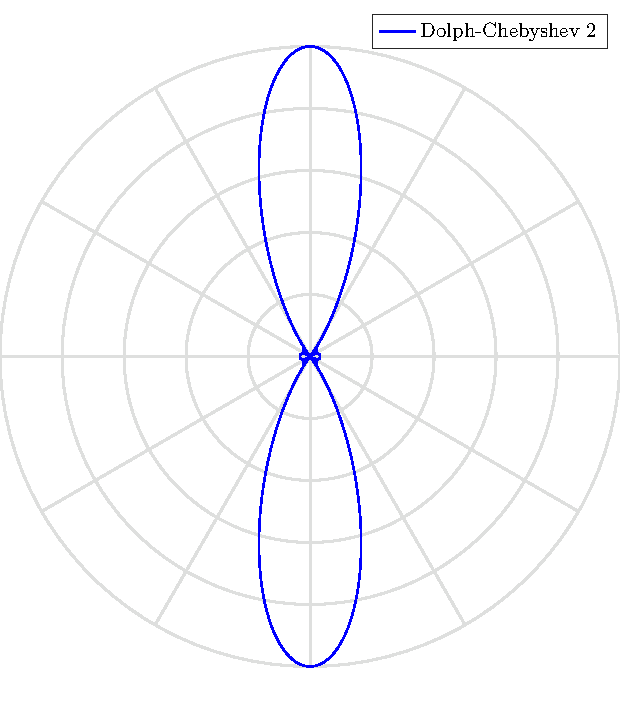
\includegraphics[width=.45\textwidth]{dc2.pdf
        }
        \label{fig:field_at_60}}
      \end{figure}
\end{frame}

% \begin{frame}[fragile]
%     \frametitle{Final Expressions}
%     \begin{figure}[h!]
%         \centering
%         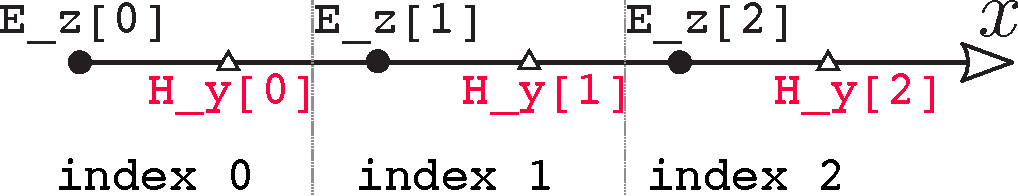
\includegraphics[width=.7\textwidth]{code_fdtd_1d.pdf}
%         \caption{Array variable definition for 1D FDTD.}
%     \end{figure}
%     The update equations for a computer program therefore are:
%     \begin{minted}{python}
%     hy[i] = hy[i] + (ez[i + 1] - ez[i]) / imp0

%     ez[i] = ez[i] + (hy[i] - hy[i - 1]) * imp0
% \end{minted}
%     Here \texttt{imp0} is the characteristic impedance, and $S_c = 1$ is assumed 1. Note the magnetic field is calculated first and then the electric field. We place the expressions above in a loop.
% \end{frame}



% %% example of an ANIMATED FRAME
% % \begin{frame}

% %         \begin{animateinline}[autoplay]{20}
% %             \multiframe{21}{rXmax=0+0.1}{
% %               \begin{tikzpicture}
% %               \begin{axis}[
% %                 axis lines=center,
% %                 domain=0.001:\rXmax,
% %                 xtick={0,1,...,8},
% %                 xmax=8.4,
% %                 ymax=1.6,
% %                 samples=51
% %               ]
% %               \addplot [gray, dashed] {1};

% %               \addplot [color=red] {1-exp(-x)*cos(3*deg(x))};

% %               \end{axis}
% %               \end{tikzpicture}
% %             }
% %             \end{animateinline}

% %   \end{frame}


\end{document}
